%!TEX encoding = UTF-8 Unicode
\documentclass[
	a4paper,
	twoside,
	justified
]{tufte-handout}
\usepackage{../../common/common}
\usetikzlibrary{automata}
%\usepackage{subfiles}
\usepackage{siunitx}
%\usepackage[options]{natbib}
\renewcommand{\rmdefault}{pplx}\usetikzlibrary{plotmarks}
\usetikzlibrary{arrows.meta}
\usetikzlibrary{decorations.pathreplacing}

\bibliographystyle{alpha}

\setcounter{secnumdepth}{1}

\title{Respostes a les preguntes \\
				sobre el TFG}
\date{29 de gener del 2015}
\author{Armand Adroher Salvia\\
	{\it UOC - TFG - EDM\&LA}}
 
\begin{document}

\maketitle

\noindent A l'atenció de Ramon Caihuelas i Julià Minguillón.

\noindent Benvolguts,
 
Us envio aquest document en motiu de les preguntes rebudes sobre la meva presentació del Treball de Fi de Grau \emph{Patrons de Connexió al CV de la UOC}. En primer lloc les reprodueixo. Seguidament miro de donar-hi resposta.

{\itshape
\begin{enumerate}[(1)]
  \item \label{q:1}  
  Quins models has deixat de banda i perquè? Per exemple, has provat o pensat a construir un model lineal generalitzat per predir si un estudiant es connectarà el dia N a partir de les dades dels dies $1,\ldots,N-1$?
  \item \label{q:2} 
  En relació a la qüestió anterior, si volem detectar des del punt de vista del docent quan un estudiant queda ``despenjat'' en funció de l’ús del campus virtual, quins models podem construir (o has construït) que consideres més adequats?
  \item \label{q:3}
  Pel que fa als perfils observats, has mirat de contrastar-los amb la literatura existent al respecte? Pots concretar una mica si us plau com has atorgat els noms a cadascuna de les tipologies detectades?
  \item  \label{q:4} 
  Finalment, resumint-ho tot, com creus que hauria d’abordar-se el problema de construir un sistema d’alertes per a que els professors tinguessin una idea clara de com va cada estudiant després del primer mes, per exemple?  
\end{enumerate}
}

Abans d'abordar directament aquestes preguntes caldria posar la totalitat del treball en el seu context. Com explico al capítol $2$ del treball, les dades que vaig rebre presenten diversos inconvenients. Amb tot, han estat els dos següents els que m'han suposat una autèntica dificultat a l'hora de mirar d'extraure'n conclusions per a la \emph{EDM\&LA}.   

\begin{enumerate}[(a)]

  \item Ha estat impossible saber quins valors de \mt{user\_id} corresponen a estudiants d'un curs semestral de la UOC, que són els que interessaven per a l'objectiu de l'estudi. En realitat, no he disposat de \emph{cap} informació en relació a aquest aspecte. En particular, no hem pogut saber quina fou, aquell semestre, o quina és, de mitjana, la proporció d'usuaris del CV que són estudiants.  
  
  \item Com, d'altra banda, explico al capítol 4, la informació que proporciona cada una de les entrades del \emph{log} que vaig rebre és en realitat molt minsa, pel que fa poder arribar a dir quelcom de significatiu sobre el comportament dels estudiants (com he dit, una part desconeguda dels usuaris) en el context del procés d'aprenentatge. És a dir, de l'esquema
  $$
    \langle \mt{user\_id}, \mt{session\_start}, \mt{last\_request}, \mt{session\_expiration} \rangle
  $$
  ja d'entrada, el \emph{timestamp} \mt{session\_expiration} només aporta informació sobre els aspectes tècnic de la relació entre l'amfitrió client i el servidor del CV, dels quals, per cert, tampoc n'he pogut saber res. Dels altres tres, \mt{session\_start} i \mt{last\_request} certifiquen que un amfitrió client identificat per mitjà de \mt{user\_id} ha enviat una petició al programari del CV, però \emph{poca cosa més ens diuen} a part de la situació de la sessión en el despregament temporal del semestre. En particular, és important no assumir res pel que fa l'activitat de l'usuari entre aquests dos instants.    
          
\end{enumerate}

Aquest fet ha provocat que dediqui una part gens menypreable del temps de què disposava per a dur a terme el TFG a mirar d'escatir de quina manera podia obtenir informació rellevant a partir d'aquestes dades, és per això que he inclòs la mètrica de presència/absència per interval de temps com a resultat notable en el primer dels subpunts de les conclusions (capítol 6). Ben bé la meitat de l'esforç invertit l'he dedicat a buscar correlacions entre estadístics derivats d'aquestes dades, tot introduint-hi transformacions que semblaven interessants\footnote[][-5\baselineskip]{Per exemple, el fet que hi hagi sessions d'un mateix usuari que es solapin em va portar de corcoll. En cert punt de l'evolucaió de l'estudi, vaig decidir que per a cada usuari, calia unificar en una de sola totes les sessions tals que existís algun segon $t$ inclòs en l'interval \mt{activity\_duration} de totes elles. Només dur a terme aquesta tasca va requerir, amb R, $65\text{h}$ de temps de CPU.}, per a comprovar, una vegada rere l'altra, que a partir dels resultats obtinguts no se'n podien deduir constatacions gaire valuoses\footnote[][\baselineskip]{Per posar un altre cas, com a conseqüència de les dues dificultats que acabo d'anotar, així com de les altres que s'indiquen en el capítol 2 de la memòria, tant el nombre de sessions per unitat de temps corresponents a un usuari, com la suma total de les duracions dels intervals, com l'hora del dia en què tenen lloc, serveixen ben poc en realitat per a caracteritzar-ne el comportament en el marc de la \emph{EDM\&LA}}.

Així doncs, pel que fa la \textbf{pregunta \ref{q:1}}, podem començar considerant com a descartats tot aquells models que havia mirat de trobar a partir de camps derivats de cada usuari, que consistien en resums estadístics dels valors de les variables corresponens a les sessions que els pertanyen. Una vegada caracteritzats mitjançant la mètrica presència/absència per interval de temps, podem distingir entre els mètodes de descobriment de \emph{clusters} i els de classificació.     

Pel que fa els mètodes d'agregació, en realitat no n'he considerat seriosament cap altre llevat dels dos que es poden apreciar al capítol 5 de la memòria, és a dir, $k$-means per als valors dels atributs $a_0, \ldots, a_m$ corresponents a cada usuari i una agregació jeràrquica amb enllaç complet a partir dels mateixos atributs de cada un dels $k$ centroides obtinguts. Havien de servir per a descobrir patrons en les dades i, a part de proporcionar una tipologia (més sobre això més avall), orientar la meva cerca. No he trobat implementacions d'agregació jeràrquica que se les poguéssin haver sense problemes amb desenes de milers d'instàncies, com és el cas dels usuaris ($\approx 75\text{K}$). Per altra banda, la cerca de nous mètodes no ha anat més enllà perquè, tot i que a la memòria només hi ocupi 8 pàgines era la possibilitat d'establir prediccions reeixides el que m'interessava. 

En relació als models de predicció el camí que he seguit ha estat una mica més llarg (i tortuós). Pel que fa les classes amb què etiquetar cada un dels usuaris, des de la decisió de l'ús de la presència per unitat de temps com a mètrica que quedava clar que qualsevol pregunta interessant a intentar respondre havia de gravitar al voltant de la qüestió de l'abandonament de la relació dels usuaris amb el CV, moment que coneixem per mitjà del darrer intèrval en què ha estat actiu. En un primer moment vaig intentar marcar un interval $I_l$ tal que poguem considerar que els usuaris en què $\mt{l\_sess} \in I_l$ (o $I_{l+1}$) han abandonat prematurament. Això no obstant, ja sigui triant aquest interval \emph{a ull} \footnote{Tot decidint, per exemple, que el punt de tall cau a una setmana abans de Nadal} com fent-ho a partir de la distribució dels valors d'aquesta variable \footnote{Triant, posem per cas, un dels seus quantils com a límit}, aquest criteri sempre m'ha semblat massa gratuït. Això es deu al fet que el concepte de \emph{prematur} no està ben definit, i menys en la situació en què ens trobem, en què no coneixem la naturalesa dels cursos \footnote{Data de la darrera PAC, presència o absència d'exàmens, etc.} que segueixen aquells usuaris que són estudiants. L'excurs del punt 5.2 de la memòria il·lustra aquest fet.                

És a partir d'aquest moment que queda clar que s'ha de fer una predicció gradual per a cada interval $n$ partir dels valors booleans corresponents dies $1,\ldots,n-1$. En aquesta direcció, si que recordo haver fet algunes proves amb models lineals generalitats. En particular per mitjà de la funció \mt{glm} de paquet base del programari R tot especificant la distribució binomial (cada $a_j$ presenta una distribució de Bernoulli) i la funció \emph{logit} (la inversa del sigmoide) com a enllaç. Però, tot reexecutant el codi he recordat que se'm queixa que l'algoritme no convergeix. Pel que vaig poder entendre, això té a veure amb el fenomen de Hauck-Donner \citep[p. 197–8]{venables02}, però anava massa curt de temps com per a aturar-me a entendre bé la qüestió i vaig prescindir-ne.   

Per altra banda, un model de predicció que sí que vaig fer servir és el de \emph{Bayes ingenu} (\emph{Naive Bayes}), ja que es cenyeix a les limitació dels meus coneixements i, a més, en domino el comportament ja que és un dels que vam emprar a les assignatures d'aprenentages computacional i mineria de dades. Intuïtivament, sembla adequat mirar de predir si en el pròxim interval temporal un usuari ja haurà abandonat o no per mitjà de l'estimació de $P(a_n|a_{n-1}, \ldots, a_0)$. Això no obstant, el model de predicció obtingut per mitjà d'aquest mètode\footnote{Mitjançant la implementació que brinda el paquet \mt{e1017} \citep{meyer14} amb un suavitzat de Laplace $\alpha = 1/100$.} és en general pitjor que el que m'han proporcionat més tard els models ocults de Markov. A la figura \ref{graph:naive_bayes_pred} hi ha una gràfica de l'evolució de certs valors derivats de les matrius de confusió corresponents a cada dia i a la \ref{graph:naive_bayes_week_pred} la dels corresponents a cada setmana.     

\begin{figure}
\begin{center}
  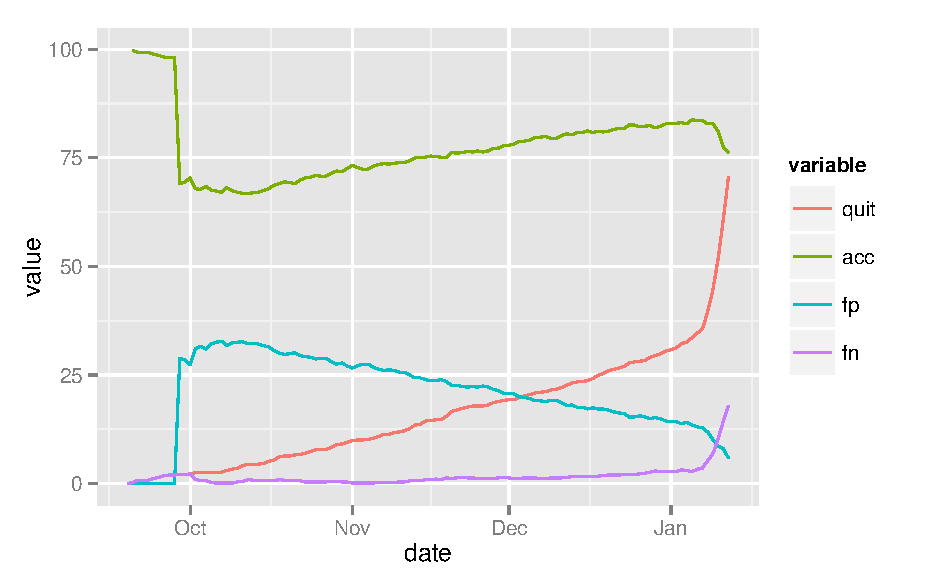
\includegraphics[width=10cm]{naive_bayes_pred}
  \caption{
    \label{graph:naive_bayes_pred}
    Evolució de la matriu de confusió per al classificador \emph{Bayes Ingenu} per $d=\text{1 dia}$.
  }
\end{center}
\end{figure}

La veritat és que ara me n'adono que, pel que fa la discretització en dies, la grafica \ref{graph:naive_bayes_pred} i  la de la figura $6.6$ de la memòria són gairebé idèntiques\footnote{La que adjunto aquí no arriba a final de semestre perquè la vaig redibuixar ahir a la tarda i havia problemes amb les dades dels darrers dies que hi havia desades a l'entorn de R desat i no era a temps de regenerar-lo }. En canvi, la de la figura \ref{graph:naive_bayes_pred} i al de la $6.7$ de la memòria presenten una divergència notable, en favor de la segona. Ara no sóc capaç d'explicar aquest fenomen i això no m'agrada. 

\begin{figure}
\begin{center}
  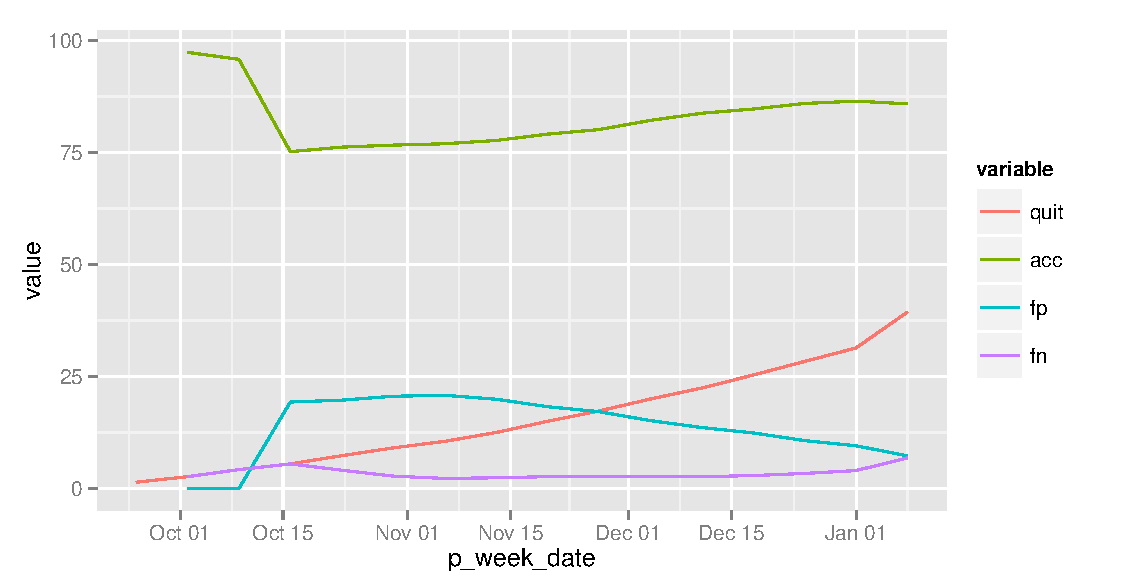
\includegraphics[width=10cm]{naive_bayes_week_pred}
  \caption{
    \label{graph:naive_bayes_week_pred}
    Evolució de la matriu de confusió per al classificador \emph{Bayes Ingenu} per $d=\text{1 setmana}$.
  }
\end{center}
\end{figure}

De fet, i ja responent la \textbf{pregunta \ref{q:2}}, ha estat caure en les cadenes de Markov de temps discret (DTMC) que m'ha fet pensar que podien ésser un bon model per a un procés estocàstic com el que en realitat és la seqüència de variables $a_0,\ldots,a_m$. Com es pot veure, per aquí van els trets a l'inici del capítol 6 de la memòria. Ara bé, el coneixement sobre la qüestió era més aviat minso, així que, tot començant per l'ubic manual de Russell i Norvig \citep{russell09} i consultant altres fonts es com vaig anar a parar als models ocults de Markov (HMM). Aquest model m'ha sembla especialment afortunat per les raons següents:

\begin{enumerate}[(a)]
  \item Permet representar el fet que en realitat \emph{mai observem a priori} (això és, abans que hagi acabat el semestre) si un usuari ja no es connectarà més al CV. Les cadenes DTMC planes de només \emph{dos estats} no poden modelar aquest fenomen encara que n'augmentem el grau o les fem heterogènies en el temps. Suposo que es podria fer tot construint nous estats en funció dels valors de $a_0,\ldots,a_{n-1}$ però estic convençut que, en créixer exponencialment,complicaria innecessàriament el sistema.
  \item Per la mateixa definició dels dos estats $A$ (actiu) i $Q$ (abandonat) ja sabem els valors de dues de les quatre transicions entre estats i de dues de les quatre probabilitats d'emissions per estat. En efecte $P(A|Q)=0$ i $P(1|A) = 0$. En haver reduït tan els estats com els valors a emetre a només 2, restem amb matrius de $2^2 = 4$ elements i, per la regla de la suma, reduïm els paràmetres a estimar també a només 2. 
  \item En darrer lloc, el model funciona igualment bé per a tots els usuaris, i no hem de suposar pel que fa si corresponen o no a estudiants (cosa que, amb les dades de què disposem, no podem fer).       
\end{enumerate}

El que sí que he d'admetre és que el mètode, d'ortodòxia dubtosa, d'estimació dels dos paràmetres d'aquest model, que s'exposa al punt 6.2 de la memòria, va ser el primer que vaig provar. En vistes dels bons resultats pel que fa les setmanes i de la limitació temporal en què em trobava, vaig decidir aturar-me aquí. Per consegüent, en relació a la pregunta, entenc que el HMM amb discretització temporal per setmanes és el model més adequat per a que el docent pugui predir que l'alumne s'ha ``despenjat''. Per altra banda, val a dir que he emprat l'algoritme de Viterbi per a fer aquesta predicció, ja que era el que tenia més a mà \citep{himmelmann10},  però en realitat proporciona més informació de la necessària i n'hi hauria hagut prou amb l'algoritme d'avenç (\emph{forward algorithm}). En darrer lloc, entenc que si volguéssim afinar més els paràmetres del model, en especial pel cas de la discretització en dies, que és el que ha sortit menys acurat, podríem fer-ho per mitjà de l'algoritme de Baum-Welch. Amb tot, dubto que en aquest cas s'arribi a cotes tan altes com en el cas de les setmanes ja que els cicles setmanas introdueixen soroll.


En tercer lloc, pel que fa la \textbf{pregunta \ref{q:3}}, la meva recerca pel que fa la literatura sobre la qüestió s'ha basat en consultar totes aquelles fonts de les referències de article de Romero i Ventura \citep{romero10} de les quals els autors diuen que han dut a terme processos de \emph{clustering}. Això no obstant, no he trobat una classificació general de tipus d'estudiant per a casos d'estudi que s'atenguin a llur presència en un entorn d'\emph{e-learning}. Els paràmetres a mesurar quasi sempre inclouen el contingut de les sessions en una aplicació web\footnote{Per exemple, el camí en el graf d'URL's} i, sí, a vegades el posen en relació amb el temps de permanència. Per acabar-ho d'adobar, en tots ells es suposa (espero que correctament) que se sap que tots els usuaris són en efecte estudiants, com és natural, ja que és d'esperar que la qualitat de les dades amb què han treballat aquests estudis sigui considerablement superior a aquelles de què he pogut disposar jo. De fet, val a dir que he encarat aquest TFG com un desafiament per a descobrir patrons en seqüències booleanes temporals en general, tot podent dir alguna cosa, per poca que sigui, en benefici de la \emph{EDM\&LA}. Però tanmateix cal admetre que el valor d'un estudi com aquest és més aviat escàs en el marc d'aquesta disciplina, a causa de la pobresa significativa de les dades en què es sustenta.

És a causa d'aquestes dificultats que la nomenclatura que he emprat en la tipologia present en el capítol 5 de la memòria és, per dir-ho així, de collita pròpia, i els diferents noms que hi apareixen no volen ser altra cosa que una abreviació substantivada de les característiques comunes de les tendències que es poden observar en els valors dels atributs dels centroides de les agregacions que subsumeixen. Dit d'una altra manera, entenc que fa la funció de simulacre de com crec que haurien d'identificar-se patrons de comportament entre els estudiants (i no en els conjunt d'usuaris en general, com és el cas ara) de tal manera que això pogués donar guies d'acció als planificadors dels plans docents per a semestres futurs. 

Per acabar, doncs, en relació a la \textbf{pregunta \ref{q:4}}, estic plenament convençut que el HMM, del qual extraure prediccions en cada moment del temps que pertanyi a l'interval corresponent segons la discretització resultant del valor de $d$ triat (és a dir, per dies o per setmanes) és una bona manera d'implementar un sistema d'avisos per a l'equip docent per tal de detectar abandonaments. És a dir, el professor pot rebre avisos de l'estil ``el sistema preveu que l'alumne $x$ ha abandonat el curs  $\{\mt{avui}|\mt{aquesta setmana}\}$''. Malgrat tot, cal notar que, a part del refinament necessari per al cas de la discretització per dia, aquest sistema encara presenta, com a mínim, els dos defectes següents:

\begin{enumerate}[(a)]
  \item Notem que, amb el que he proposat al capítol 6 de la memòria, de moment només podem saber que l'alumne \emph{acaba d'abandonar el curs}. Aquesta situació pot mirar de reconduir-se si el docent té la manera de contactar amb l'estudiant per mitjà d'una altra via que no sigui el mateix CV, és clar. Altrament, la notícia arribaria massa tard. Per resoldre aquesta mancança entenc que sí que és necessari l'ús de l'algoritme de Viterbi. Dic això perquè la primera solució que se m'acudeix passa pel següent.
  \begin{enumerate}[(i)]
  \item En primer lloc, si ens trobem en l'interval $I_n$, obtenir, per mitjà d'aquest algoritme, la sequència d'estats $x_1,\ldots,x_{n-1} \> (x_i \in \{A,Q\})$ que és més probable que hagi generat la seqüència d'emissions $y_1, \ldots, y_{n-1} \> (y_i \in \{0,1\})$ a la qual sí que hem tingut accés. 
  \item Estimar la matriu de transicions $M$ entre estats a partir de $x_1,\ldots,x_{n-1}$ per mitjà de la màxima versemblança (MLE), tal com explico al punt $6.1$ de la memòria. 
  \item Si volem saber la probabilitat de l'abandonament futur de l'alumne en l'interval $I_{n+k}$, i $\pi$ és el vector de probabilitats dels estats inicials, la calculem per mitjà del producte $\pi M^{n+k-1}$     
  \end{enumerate} 
  \item La segona mancança del sistema proposat fins ara és que no indica al professor la seguretat amb què es fa la predicció, o si es vol, la probabilitat que sigui correcta. Ara mateix no sabria apuntar per on haurien d'anar aquests càlculs.  
\end{enumerate}
           

\noindent Moltes gràcies pel vostre temps.

\noindent\rule{4cm}{0.4pt}

\bibliography{aadroher_uoc_tfg}


\end{document}

